\documentclass[11pt]{article}
\usepackage[margin=1in]{geometry}
\usepackage{amsmath,amssymb}
\usepackage{booktabs}
\usepackage{array}
\usepackage{graphicx}
\usepackage{xcolor}
\usepackage[colorlinks=true,linkcolor=blue!50!black,urlcolor=blue!50!black]{hyperref}
\usepackage{parskip}
\usepackage{float}
\newcommand{\g}{\textsf{g57}}
\newcommand{\doc}[1]{\texttt{#1}}
\newcommand{\xor}{\oplus}
\newcommand{\lgi}{\textsc{lgi}}
\newcolumntype{L}[1]{>{\raggedright\arraybackslash}p{#1}}

\title{Blinded-V5: the \lgi-based compute module\\
  \large design rationale, construction, parameters, and measurements}
\author{local-mixing project}
\date{2026-09-04}

\begin{document}
\maketitle

\section*{Where it fits in the pipeline}

A secret circuit $C$ on $n$ wires is protected in two steps: it is first
\textbf{gadgetized} into an equivalent but structurally-scrambled circuit on $2n$
wires, which is then \textbf{mixed} (fmix). Blinded-V5 lives inside the
gadgetizer, and this document assumes you know the earlier gadgetize designs but
nothing about V5.

The \textbf{gadgetize module} is a \textbf{5-stage} pipeline, each stage on $2n$
wires (data $0..n$, band/junk $n..2n$):

\begin{enumerate}
\item \textbf{slice} --- a junk-guard zero-slice keyed on the band (dead at the
  input port, where the band is 0);
\item \textbf{seed the band wires} --- each band wire set to $x_i \land \lnot x_j$
  from the honest inputs;
\item \textbf{compute} --- realise the input circuit $A$ on the $2n$ wires so the
  data half carries $A$'s output and the band is only read;
\item \textbf{re-seed / re-randomise the band wires} --- band turnover;
\item \textbf{re-slice} --- the closing junk-guard slice (fires at the output
  port).
\end{enumerate}

One term to keep straight: the circuit $A$ that the gadgetizer computes is
\textbf{not $C$ itself}. It is the \textbf{sliced sandwich of $C$} --- the output
of a \emph{separate} \textbf{sandwich module} that wraps $C$ (with a random $D$,
interleaved slice blocks, a floated column) into a $2n$-wire circuit with
$A(x,0) = (\mathit{junk}, C(x))$. The sandwich \emph{generates} the circuit that
the gadgetize module then computes and mixes; it is a different module and is not
one of the five stages above.

\textbf{Blinded-V5 is a drop-in replacement for stage 3 --- the compute.} Where
the earlier compute stages (the drip \doc{route\_fire}, the product-share
carriers) realise $A$ by \emph{routing} each operand into position and firing a
gadget there, Blinded-V5 instead embeds $A$ \textbf{inside one enormous masking
identity}: the compute's body is a cloud of long masking identities on the band,
and $A$'s gates fire from \emph{within} the mask by a momentary, reversible
unmasking of their operands. It takes $A$ and emits an equivalent $A'$ on the $2n$
wires; the other four stages are unchanged. (V5 re-randomises the band
\emph{internally} as part of its own masking hygiene --- \S2 --- which is distinct
from the separate stage-4 re-seed.)

Source: \doc{src/preprocessing/blinded\_v5.rs}. Driver:
\doc{gen\_sandwich\_gadget ... blinded-v5}; pipeline:
\doc{gss\_mix.sh -{}-gadgetization-mode blinded-v5}. The Markdown twin of this
document is \doc{BLINDED\_V5\_LGI\_DESIGN.md}.

\section{Why this design --- the rationale}

The compute stage must move the intermediate state as far as possible from the
plaintext computation $A$ while keeping $A'$ exactly equivalent to $A$ on the data
wires. The design is a chain of forced moves.

\paragraph{(a) Long identities are the only thing that moves the state.} Across
the HD and affine heatmaps, short local edits barely displace the state; the ridge
of recoverable structure only recedes when the masking identity woven through a
wire is \emph{long} --- comparable to the circuit itself.

\paragraph{(b) The only long identity that moves the state is the commutative
structure of an identity with a single active wire.} A run of gates all targeting
one active wire $w$ and reading only controls is an identity iff the increments
\textsc{xor} to zero, and \emph{all its gates commute} --- which lets it be
arbitrarily long and freely interleaved.

\paragraph{(c) Entangle identities on different active wires by sharing the
control wires --- the band.} Every identity targets a data wire and reads only the
band ($n..2n$), so identities on different active wires also commute; a band wire
participates in the masks of many data wires at once.

\paragraph{(d) Add random updates of the control wires from the active wires ---
in bursts.} Band updates \textbf{re-randomise} the controls (fresh band entropy
throughout the run, not just at the seed) and \textbf{break naive commutation-back}
(once a band wire is updated mid-run, the identities reading it before and after no
longer commute past it), without ruining correctness (each straddling identity is
closed before the update or re-derived across it). The updates are emitted in
\textbf{bursts}: one \emph{slot} is $F \approx 8\mathrm{K}$ gates all targeting a
single band wire $b$, each control drawn independently as a live-data or a band wire
(so a burst spans $b \mathrel{\xor}= \mathit{data} \land \mathit{aux}$, $b
\mathrel{\xor}= \mathit{aux} \land \mathit{aux}$, and $b \mathrel{\xor}= \mathit{data}
\land \mathit{data}$). Bursting \textbf{concentrates} the band mixing into few slots
(so fewer straddle-closures interfere with the \lgi s) and gives each band wire a
\textbf{data-wire-like burst-of-activity signature}.

\paragraph{(e) Embed $A$ inside one circuit-spanning identity via hidden
unmasking.} Each gate fires from inside the mask: its operands are momentarily and
reversibly unmasked into a linear combination of band wires (never bare), it fires
as an expansion over those masked wires, then re-masks.

That is the whole design: a long, entangled, self-updating masking cloud with $A$
firing from inside it. Everything in \S2 is \emph{how} to realise (a)--(e) as a
single correct circuit.

\section{The construction}

$A$ has $n$ wires and $m$ gates; $A'$ has $2n$. Let $u_w$ be the uses of wire $w$
in $A$ and $w_w$ its writes.

\paragraph{Masking atom.} $\g(w,x,y) = w \mathrel{\xor}= 1 \xor (\lnot x \land y)$
(data target, band controls), i.e.\ the mask term $1 \xor y \xor xy$. A
disjoint-pair \lgi{} $\bigoplus_i \g(w, cy_{2i}, cy_{2i+1})$ is a deg-2 mask; a \g{}
and its reverse \textbf{linearise}, $\g(w,r_1,r_2) \xor \g(w,r_2,r_1) = w \xor r_1
\xor r_2$ --- the original read exploited this; the current read
(\textbf{quad-fire}, step 2 below, default since 2026-09-06) deliberately does
\emph{not}, because a linearised operand is exactly affine in band wires for a window
that the pipeline's reordering stages stretch into a leak (\S5.0). Disjoint pairs,
not a $K$-cycle (which would telescope to a bare operand); $K \ge 2$.

\paragraph{Why one pass --- co-sampling.} The masks, the band updates, and $A$'s
gates are \textbf{co-sampled}: produced together in a single forward pass, rather
than laying a fixed masking scaffold first and threading $A$ through it afterwards.
The reason is hidden firing (\S3): every $A$-gate must be straddled by a
\emph{real}, rerand-protected masking identity opened at the exact instant the gate
fires. Only a co-sampled pass can open that identity on demand, so the
firing-hiding is complete while reusing the wire's existing mask budget --- at no
size cost. (A fixed scaffold, filled in afterwards, starves at the tail and covers
only 60--70\% of gates; \S3.)

\paragraph{The algorithm.} A cheap setup, then a forward pass.

\emph{Setup.}
\begin{enumerate}
\item \textbf{Mask budget.} Give each active wire $w$ exactly $u_w+1$ masking
  identities, split into $w_w$ \textbf{straddle opens} (one per write to $w$,
  opened \emph{on demand} at the gate that writes it --- for hidden firing) and
  $\mathrm{reads}_w+1$ \textbf{filler opens} (opened between gates to keep $w$
  masked while it is read). At most \doc{max\_open} are open on a wire at once.
  This is the same budget a fixed scaffold would use, so the statistics are
  unchanged.
\item \textbf{Order.} Build the data-hazard DAG of $A$ (\doc{compute\_deps}): a
  read is ordered after every earlier write of the wire, and a write after every
  earlier read --- but same-target XOR writes commute, so there is \emph{no}
  write-after-write edge. Any linear extension preserves $A$'s function; a Kahn
  \textbf{ready queue} holds the gates whose predecessors are all placed.
\item \textbf{Rerand plan.} A shuffled list of \doc{straddle\_slots} $+$
  \doc{repair\_slots} band-update \emph{slots} (\S1d; auto \doc{straddle\_slots}
  $\approx m/(4K)$, \doc{repair\_slots} $= 0$).
\item \textbf{Rate.} Fire one rerand slot every
  $\mathit{total\_steps}/\#\mathit{slots}$ primitive steps (a \emph{step} $=$ one
  $A$-gate placement or one filler open; $\mathit{total\_steps} = m +
  \Sigma\,\mathrm{filler}$), so the slots spread evenly and the last lands
  \emph{during} the pass --- no end-flush (a surplus of requested slots over
  $\mathit{total\_steps}$ warns rather than truncating silently).
\end{enumerate}

\emph{Forward pass} --- repeat until all $m$ gates are placed:
\begin{enumerate}
\item \textbf{Pop} a ready $A$-gate $g$ (target wire $c$).
\item \textbf{Masked read (quad-fire).} For each operand wire, leave its
  currently-open masks \emph{as they are} and describe the wire as the ANF
  polynomial $P_w = w' \xor \sum_{(x,y)} (1 \xor y \xor xy)$ over its net-open pairs
  (a pair whose reverse is also open contributes the linear $x \xor y$); top up with
  \textbf{fresh single \g s} (quadratic, not pair-completed) until at least
  \doc{max\_open} quadratic terms mask the operand (the \textbf{hard floor}: never
  bare, never affine). Remember the top-up gates as the \emph{undo} --- except that
  an operand with \textbf{no open \lgi{} at all} keeps its first top-up as a real
  \lgi{} (the \emph{read-cover} rule, \S5.6: otherwise a seldom-used wire returns to
  holding its plain value for the whole idle stretch after the fire). (Legacy linear
  read, \doc{BV5\_QUAD\_FIRE=0}: complete each open \g{} with its reverse so the wire
  carries $\mathit{operand} \xor \rho$, $\rho$ a linear \textsc{xor} of band wires,
  top up with pairs until $|\rho| \ge \doc{min\_mask}$, undo the reverses after the
  fire --- see \S5.0 for why it was replaced.)
\item \textbf{Fire from inside the mask.} Expand $c \mathrel{\xor}= \mathit{comp}
  \xor \mathrm{lit}(a)\land\mathrm{lit}(b)$ as the polynomial product $P_a \cdot P_b$
  (a negative literal complements the constant) into a batch of monomials over
  \textsc{only} the masked control wires and band wires --- never bare $a$, $b$, or
  $a\xor b$ (0/1/2 controls and all polarities; the 0-control fire is
  $\lnot\mathit{comp}$). At $K=2$, \doc{max\_open}$=3$ that is up to $8\times8=64$
  monomials of degree $\le 4$ (versus 49 of degree 2 plus the linearise/undo bracket
  in the legacy read), so the gadget is ${\sim}12\%$ \emph{smaller}.
\item \textbf{Straddle (hidden firing, \S3).} Split the monomial batch into two
  halves, shuffle each \textbf{independently} (they all target $c$ and commute),
  emit the first half, \textbf{open a fresh \lgi{} on $c$ here} (one of its straddle
  opens, generated on demand), then emit the second half. The mid-fire open makes
  the module's net XOR on $c$ equal $\Delta \xor \text{secret-mask}$, not the bare
  increment $\Delta$.
  The whole block is \textbf{bracketed by a temporary cover mask on $c$} drawn
  away from every band wire of the operands' polynomials (opened before the
  first monomial, closed after the last; the straddle open is drawn away from
  those wires too): a band wire shared between one of $c$'s masks and a fire
  monomial would cancel or fold that mask's uniform term and leave the mid-fire
  segments biased toward $c_{\mathrm{new}}$ (\S5.7; ${\sim}6$ gates per fire,
  ${\approx}3\%$).
\item \textbf{Undo} --- emit the top-up gates again (each is an involution),
  restoring the operands' original mask set.
\item \textbf{Maybe rerand} --- if the calibrated rate says so, emit one
  band-update slot (below).
\item \textbf{Release \& fill} --- decrement the in-degree of $g$'s dependents,
  moving any that reach zero into the ready queue; then open a few \textbf{filler}
  \lgi s on wires chosen by remaining filler budget.
\end{enumerate}

\emph{Finish.} Drain any remaining filler opens, then close every still-open
\lgi{} so the data wires end holding $A$'s true output.

\paragraph{The rerand slot} (step 6) is a \S1d burst: one band wire $b$,
$F \approx 8\mathrm{K}$ updates. A \textsc{straddle} slot first \textbf{closes} the
masks reading $b$ (this is what thins masking past the $\approx1024$ knee --- hence
keeping \doc{straddle\_slots} at that budget); a \textsc{repair} slot brackets the
burst with each such mask's $b$-reading \g{} (old $b$ cancels, new $b$ re-adds, so
the mask stays open --- no thinning). Running in the same pass, the band updates
protect the straddle opens automatically. \textbf{Coverage across the burst is a
rule, not a statistic:} when the masks reading $b$ are \emph{all} of a wire's open
masks, the slot first opens a \emph{replacement} \lgi{} on that wire (sampled away
from $b$) and only then closes them --- same-target \textsc{xor} writes commute, so
open-then-close never leaves an instant with no mask on the wire. Without it the
wire sat bare, holding its plaintext value, until its next filler (\S5.6: every
interior bare interval of the earlier builds came from this --- ${\sim}450$ per
build, median ${\sim}10^4$ gates). Every \lgi{} sample (fillers, straddle opens,
replacements, read top-ups) also draws its band wires \textbf{disjoint from every
band wire already used by the wire's open masks}. Any shared wire biases the mask
sum: two identical pairs cancel ($1\xor y\xor xy$ twice is 0 --- the wire is
functionally bare while the bookkeeping counts two masks), two identical balancing
wires cancel ($z\xor z=0$, no uniform term left), and a balancing wire equal to
another open pair's wire folds the linear and the quadratic term into an
\textsc{or} ($x \xor \neg x{\wedge}y = x\vee y$, biased 3:1). Each of these showed up
as a phi ${\approx}0.25$ segment population in the gauntlet at 32 band wires
(\S5.7); at 256 the last one still hits ${\sim}10\%$ of opens. The same discipline
applies to the \textbf{burst gates}: a burst $b \mathrel{\hat{}}= \mathit{lit}(c_1)
\wedge \mathit{lit}(c_2)$ with a data control reads that wire under its masks, so
its other control is drawn away from that wire's mask wires (and two data
controls may not share a mask wire) --- otherwise the product strips a mask's
uniform term and the burst's flip correlates with the plaintext (phi 0.14--0.26,
seen at \doc{max\_open}~2, \S5.7).

\paragraph{Correctness} is verified exhaustively over all $2^n$ inputs $\times$
many band settings for $n \le 6$, $K \in 2..5$, all \doc{max\_open} and both
rerand kinds (\doc{scratchpad/v6}: 891 gadgets, 0 mismatches, plus a 360-case
reorder-preserves-$A$ check; the linear read), by the unit test in
\doc{blinded\_v5.rs} ($n=6$, all $2^n$ inputs $\times$ 8 band states $\times$ 6
seeds, \textbf{both read modes}), and end-to-end in \doc{gen\_sandwich\_gadget}
(forward + reverse-honesty sample-verify PASS in both modes).

\section{Hidden firing}

An \emph{atomic}, mask-restoring gate module would leak which gate fired: the
active wire's before/after XOR across it equals the true increment $\Delta =
\mathit{comp} \xor \mathrm{lit}(a)\land\mathrm{lit}(b)$. That per-module increment
is a robust invariant that survives the downstream mixing, so an adversary who
segments the mixed circuit at module boundaries reads off $A$'s gate list.

The fix uses the abundant masking gates on the \emph{same} active wire: split the
fire and emit one of $c$'s \lgi{} \textbf{opens between the halves}. It toggles
$c$ mid-fire and stays open past the module, so the net XOR on $c$ is $\Delta \xor
(\text{secret band-mask})$ --- never the bare increment. Because everything is
co-sampled, the straddling \lgi{} is a real, rerand-protected scaffold \lgi{}
opened exactly when the gate is placed, so \textbf{every} gate is covered, reusing
the wire's $u_w+1$ budget at \textbf{no size cost} (measured: 7920/7920 gates on
the n=128 sandwich). Earlier attempts --- $A$-gate weaving ($\sim$23\%), an
injected firing mask (100\% but +43\% size), straddling fixed-scaffold slots
(60--70\%, tail slot-starved) --- are superseded by generating the slot on demand.

\section{Parameters and why}

\begin{table}[H]\centering\small
\begin{tabular}{@{}lcL{3.4cm}L{5.0cm}@{}}
\toprule
knob & prod. & meaning & why this value \\
\midrule
$K$ & \textbf{2} & band wires per \lgi{} = per-\lgi{} \textbf{mask width}
  ($\lfloor K/2\rfloor$ pairs; $|\rho|\approx\doc{max\_open}\cdot K$) --- not the
  temporal length & affine/deg-2-neutral across $K$ (\S5); smallest is best. Size
  $\sim$linear, read cost quadratic in $|\rho|$, so large $K$ explodes. Odd $K$
  wastes a wire. \\
\addlinespace
\doc{max\_open} & \textbf{3} & rolling cap on simultaneously-open \lgi s per wire
  & wider $\rho$ = more local hiding, but read cost is quadratic in $|\rho|$; 3 is
  the knee. \\
\addlinespace
\doc{quad\_fire} & \textbf{on} (2026-09-06) & read operands from inside their
  quadratic masks; never linearise & the linearised read leaves the operand exactly
  affine in band wires for a window that every reordering stage stretches into the
  $C$-vs-$G$ ridge (\S5.0); quad-fire has no window, keeps the ridge at the I/O
  fringe through the whole pipeline, and is ${\sim}12\%$ smaller.
  \doc{BV5\_QUAD\_FIRE=0} $=$ legacy. \\
\addlinespace
\doc{balanced} & \textbf{on} (2026-09-07) & every \lgi{} (and
  every read top-up) adds one \textsc{cnot} $w \mathrel{\hat{}}= z$ from a fresh band
  wire, so each mask term is $z \xor 1 \xor \neg x{\wedge}y$ --- unbiased, still
  quadratic; band seed $x_i \xor x_j$ & a bare \g{} term is 1 three times in four,
  so a wire under one open mask is \emph{linearly correlated} with its plaintext
  (phi 0.29 with the $C$ gate's firing predicate; \S5.6). Balanced masks take that
  channel to the null floor (median phi 0.08) at +92\% gates ($K{=}2$,
  \doc{max\_open} 3: read polynomial $8{\times}8 \to 11{\times}11$ monomials); it is
  what passes the gauntlet's w1/w2/w3 (\S5.7). \doc{BV5\_BALANCED=0} $=$ plain masks;
  \doc{max\_open}~2 balanced is the +10\% variant, weaker against two-feature scans. \\
\addlinespace
\doc{min\_mask} & \textbf{auto\,$=\doc{max\_open}=3$} & \textbf{hard floor} per
  operand read: quadratic mask terms (quad-fire) / masking wires $|\rho|$ (legacy)
  & guarantees no operand is ever read under fewer than 3 masks, even in a rare draw
  where the open pairs cancel (legacy: worst read $|\rho|$ rises $2\to4$; mean
  $|\rho|\approx5.9$ unchanged; +0.2\% gates). \\
\addlinespace
\doc{rerand\_level} & \textbf{auto\,$=m/(4K)$} ($\approx$875) &
  close-straddling-masks band-update \textbf{slots} & at the safe side of the
  $\approx1024$ thinning knee; the \emph{slot} count (not the gate count) is what
  thins. \\
\addlinespace
\doc{rerand\_repair} & \textbf{0} & re-derive-across-update band-update slots (no
  thinning) & off by default; add slots for extra band turnover at no masking cost.
  \\
\addlinespace
\doc{rerand\_burst} ($F$) & \textbf{auto\,$=8\mathrm{K}$} (=16 at $K{=}2$) &
  band-update gates \textbf{per slot} (the burst) & comparable to a data wire's
  write-burst (tens of gates), so band wires carry a data-wire-like activity
  signature; $\mathit{slots}\times F\approx2m$. \\
\bottomrule
\end{tabular}
\end{table}
\noindent $K$ sets each \lgi's mask \emph{width}, not its temporal length --- the
identity's circuit-spanning length is a property of the whole scaffold (\S1e).

\section{Measurements}

All measurements are on the current co-sampled build with \textbf{burst rerand $+$
the masking floor} (n=128, $|C|=|D|=3000$, K=2). They match the pre-firing-fix
baseline to within noise --- neither the hidden-firing redesign nor the burst/floor
refinements moved them (the burst change touches only the band wires, so it cannot
move the data-wire ridge): degree-1 $\mathrm{meanH}=0.4966$, degree-2
$\mathrm{meanH}=0.4967$, exposed-$C<0.35\approx5.6$--$5.7\%$.

\subsection*{5.0\quad The affine ridge through the pipeline, and why the read mode changed (2026-09-06)}

The figures in \S5.1--\S5.5 were read by \textbf{mean H} and by the count of
\textbf{exposed rows} (segments with a cell below 0.25/0.35). Both are blind to a
ridge made of \emph{exact} affine relations at a few bits per cell, and the ridge
statistic of \doc{plot\_hmap\_ridge.py} (depth, median-row depth, $\rho$) had never
been computed for the pipeline circuits. Computing it showed a full-strength diagonal
in every mixed circuit of the linear-read design: the raw gadget has ${\approx}$500--800
exact relations (median-row depth 0.008 --- the ``depth $\approx 0.05$'' of \S5.1 is the
I/O fringe plus a faint trace), the 2-eff snapshot ${\approx}$6{,}000 (median-row depth
0.07, $\rho=1.00$, permutation $z=9.6$), and the compressed, packed final
${\approx}$7{,}000 (depth 0.10). Each relation is one $C$ bit equal to the XOR of the
data wire and its ${\sim}6$ linearised band wires: a \textbf{masked-read window}. The
undo of a read is a write to the operand wire, pinned only by that wire's next read, so
every reordering stage --- the DB splice moves of phase A, fmix's final uniform float,
the crossing walk --- stretches the window to the operand's idle interval (isolated:
reordering-only moves $503 \to 601$ in snapshots, the final float alone $\to 4{,}555$;
DB moves saturate by ${\approx}1$ move/gate). No parameter fixes it: extra filler
\lgi s or repair slots dilute it by ${\approx}\div2$ at $+35$--$55\%$ gates, mask width is
irrelevant, and \doc{max\_open}$=2$ is worse (full tables in
\doc{RIDGE\_QUADFIRE\_20260906.md}).

\begin{center}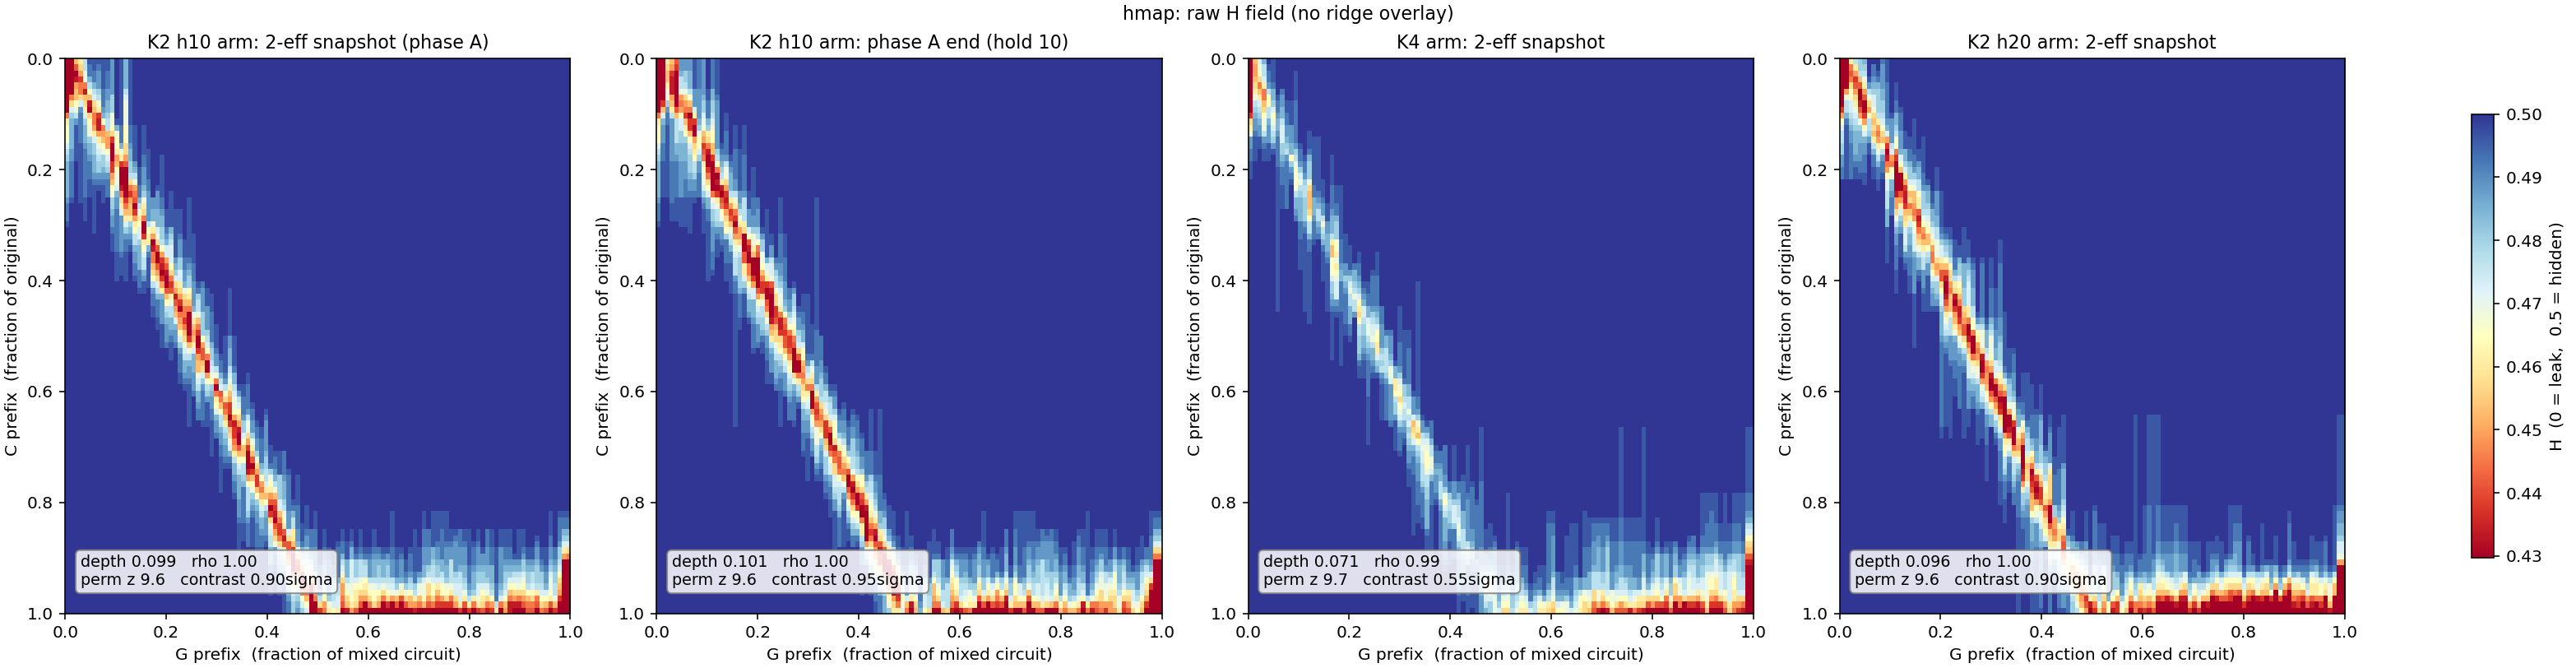
\includegraphics[width=\textwidth]{blindedv5_linear_phaseA_ridge.png}\end{center}

\textbf{Quad-fire} (\S2 step 2) removes the window instead of diluting it. Same recipe,
2-eff pipelines, exact relations per stage (depth / median-row depth):

\begin{table}[H]\centering\footnotesize
\begin{tabular}{@{}lll@{}}
\toprule
stage & linear read & quad-fire \\
\midrule
gadget & 563{,}356 g, 834 (0.049 / 0.008) & 497{,}548 g, 500 (0.048 / 0.000) \\
2-eff phase A & 962{,}429 g, 6{,}032 (0.093 / 0.066) & 898{,}416 g, 443 (0.050 / 0.004) \\
split & 1{,}839{,}248 g, 5{,}984 (0.096 / 0.070) & 1{,}507{,}931 g, 478 (0.049 / 0.004) \\
crossing & 3{,}345{,}382 g, 4{,}574 (0.081 / 0.051) & 2{,}738{,}434 g, 368 (0.049 / 0.004) \\
final (fcompress $+$ pack) & 337{,}194 packed, 7{,}179 (0.104 / 0.082, $\rho$ 1.00) & 311{,}285 packed, 400 (0.049 / 0.004) \\
\bottomrule
\end{tabular}
\end{table}

\begin{center}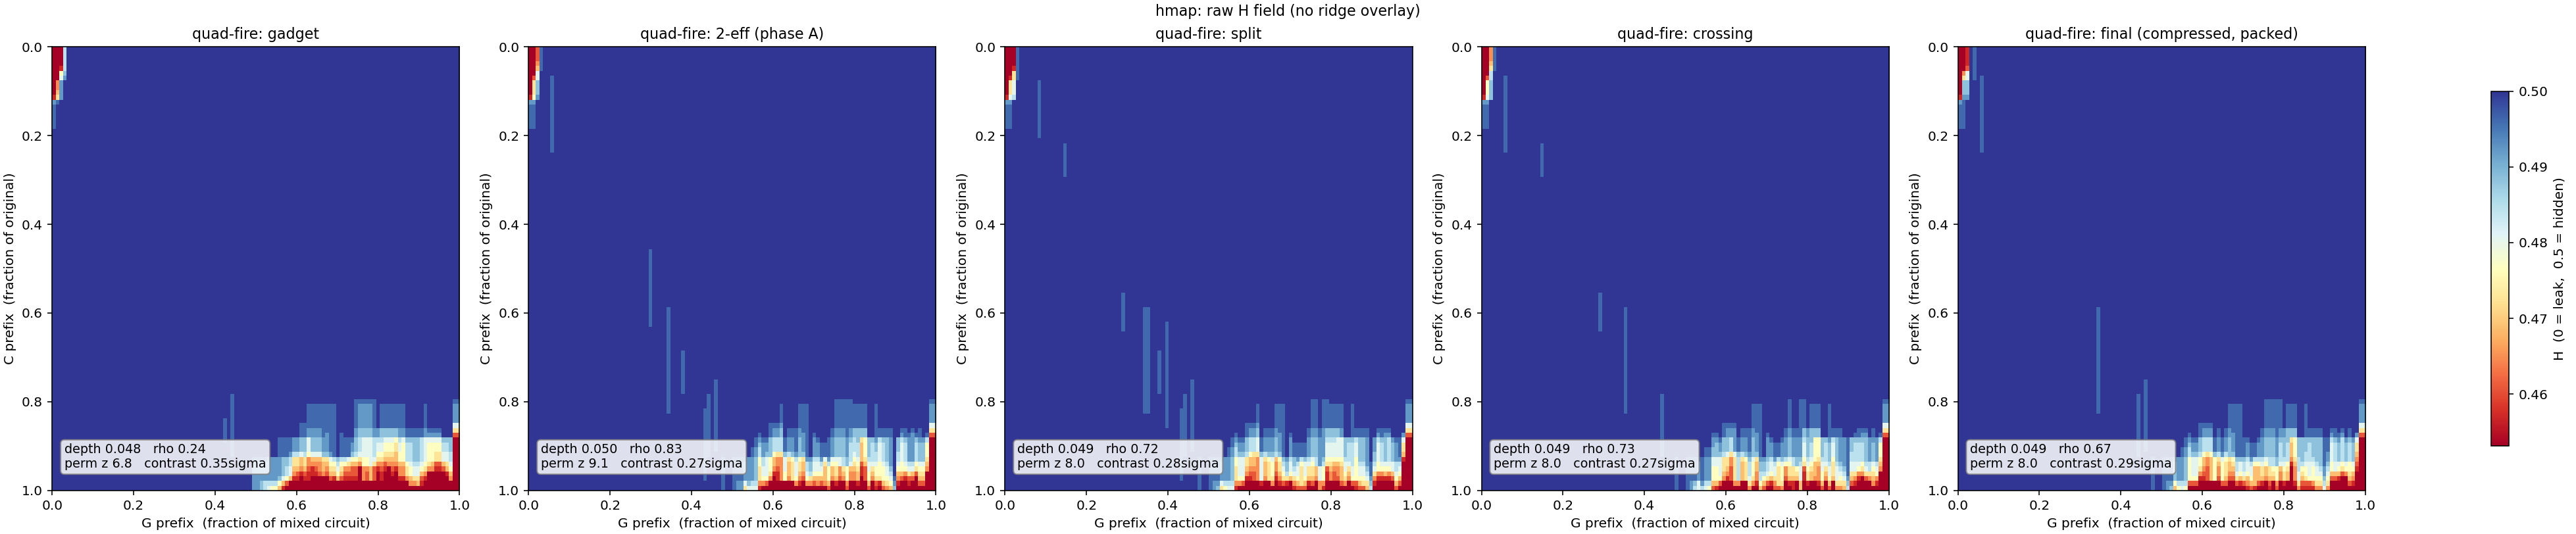
\includegraphics[width=\textwidth]{blindedv5_quad_pipeline.png}\end{center}
\begin{center}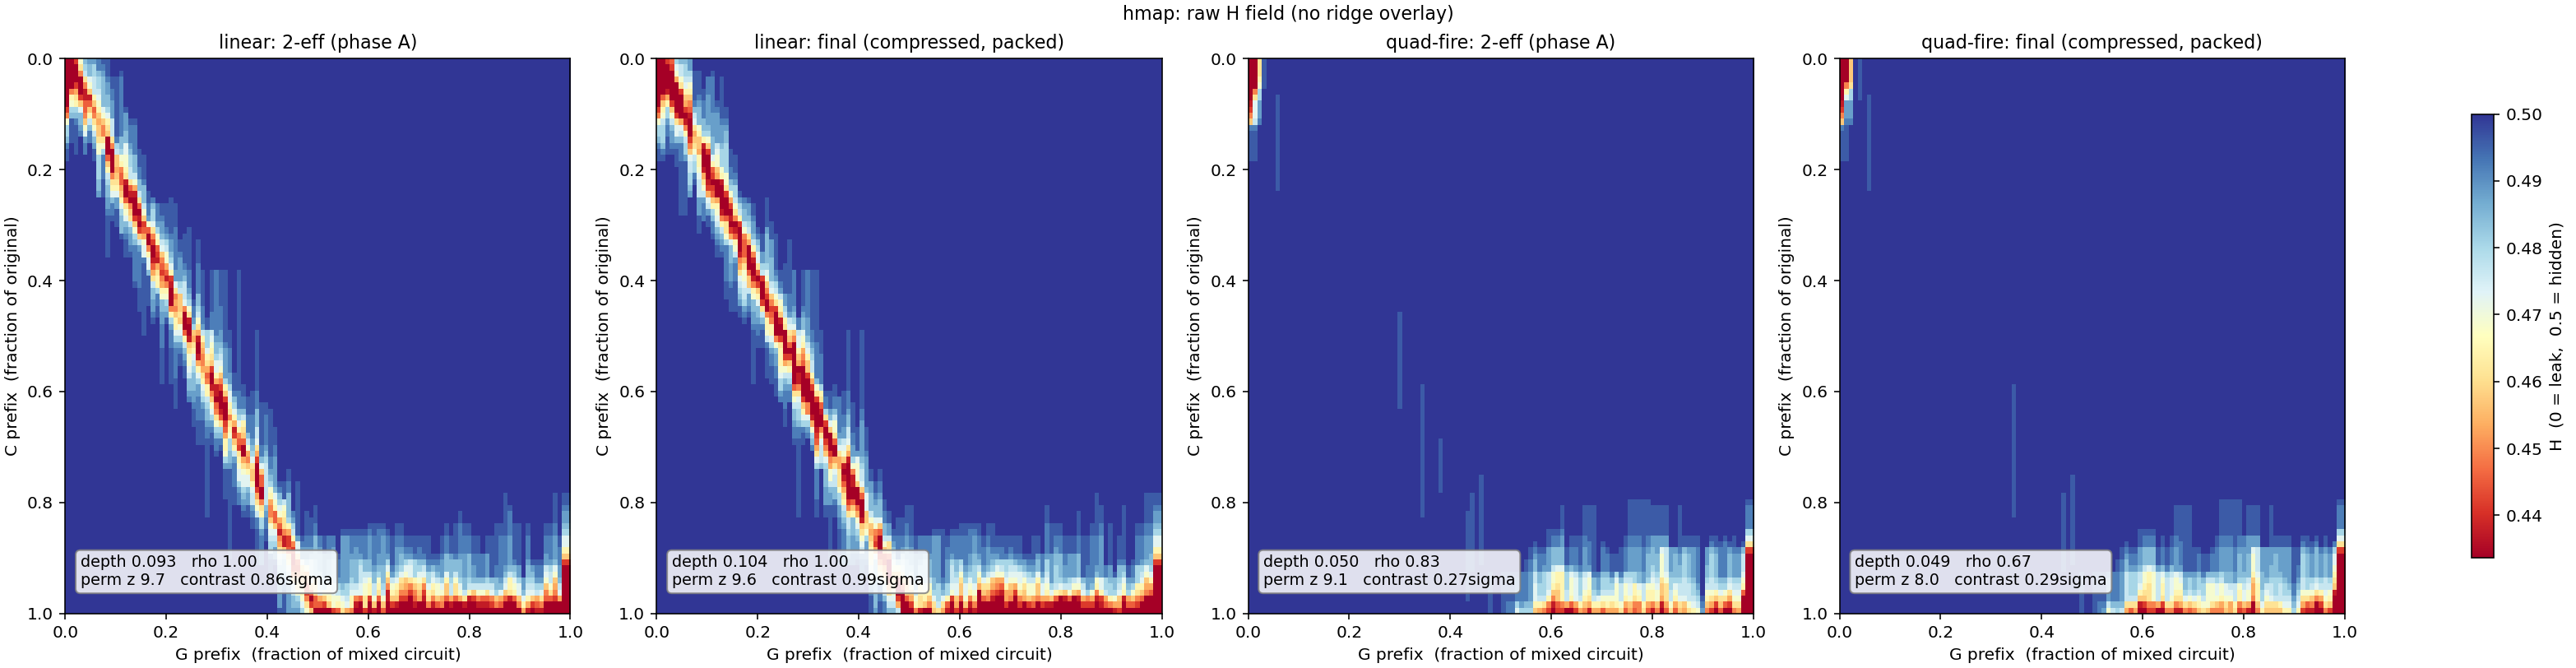
\includegraphics[width=\textwidth]{blindedv5_lin_vs_quad.png}\end{center}

The residual 150--500 relations of quad-fire are single-wire identities in the
delivered-output rows and at the raw input port --- the public I/O fringe of \S5.2 ---
and they do not grow with mixing (flat from the gadget to 3 moves/gate in phase A and
through split, crossing and compression). The degree-2 adversary of \S5.3 (products
over a 24-data $+$ 24-band slice) is likewise flat for quad-fire ($141 \to 102$ after a
float) where the linear read goes $481 \to 4{,}978$; a full degree-2 adversary with every
band-pair product would cancel three open quadratic masks in either design (the
existing sample-count-bounded posture), so quad-fire closes the affine channel, which
was the open one.

\subsection{Affine ridge --- raw gadget, linear read}

\begin{center}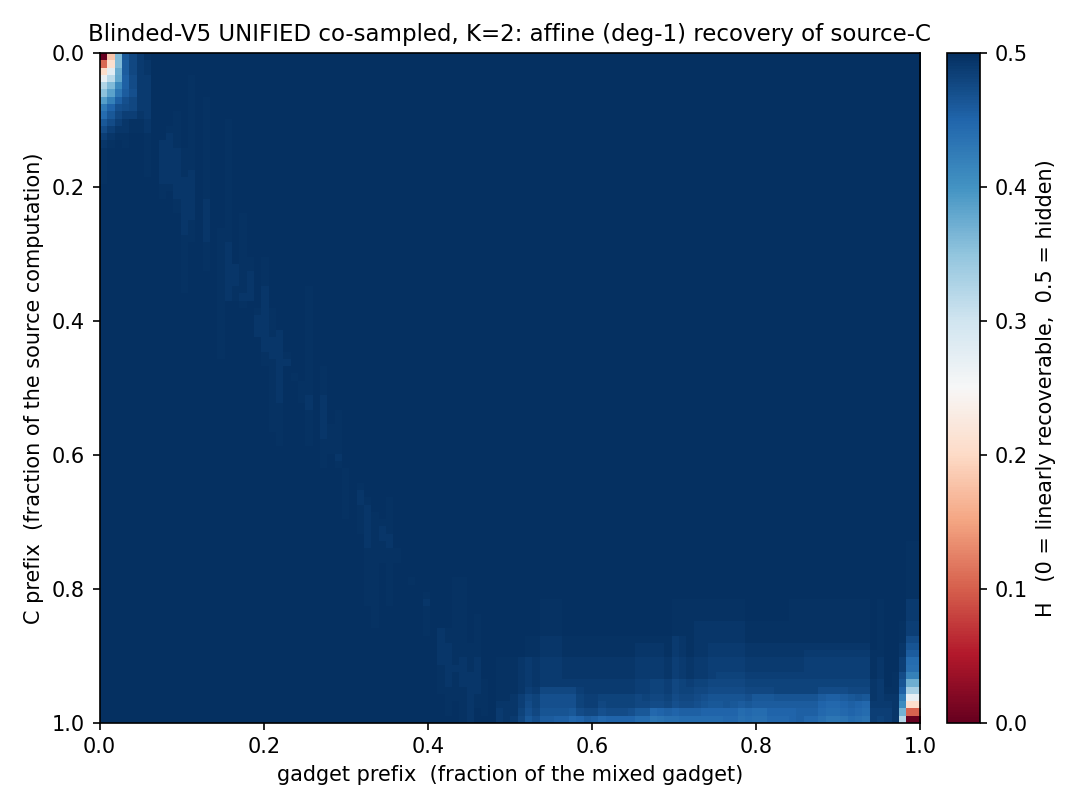
\includegraphics[width=0.82\textwidth]{blindedv5_affine.png}\end{center}
\noindent $\mathrm{meanH}\approx0.498$, ridge depth $\approx0.05$; the interior
($\sim$78\% of rows) is fully hidden ($H\approx0.49$), and the only recovery is a
thin fringe at the two endpoints.

\subsection{The exposed fringe is public I/O --- input segments are not leaked}

The $\approx$6--10\% of source-$C$ segments that are linearly exposed
($\min$-$H<0.25$--$0.35$) are the two corners of the diagonal. The \textbf{input
side is masked as soon as the compute begins} --- recovery is confined to the
extreme top-left corner, i.e. the raw input port where $x$ is public \emph{before}
any masking. The output side is the necessarily-delivered $C(x)$. So the input
wire segments show a \textbf{lack of linear exposure} beyond the trivial public
input; the boundary-cushion knobs measured no effect because the fringe is
unavoidable public I/O, not a leak.

\subsection{Degree-2 recovery}

\begin{center}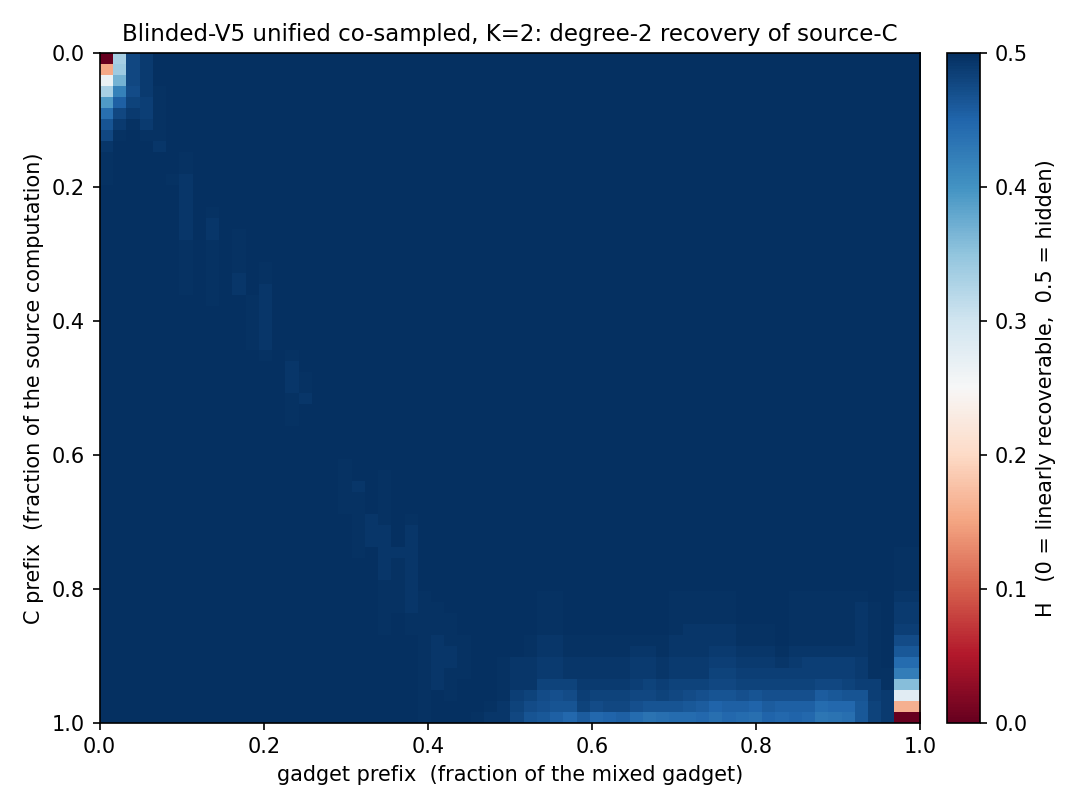
\includegraphics[width=0.82\textwidth]{blindedv5_deg2.png}\end{center}
\noindent $\mathrm{meanH}\approx0.497$, depth $\approx0.05$. The quadratic
adversary reaches only $\sim$0.01 deeper than affine, into the same low-degree I/O
fringe; the interior stays fully hidden. Degree-2 is flat across $K$, like affine.

\subsection{Rerand: bursts, straddle vs repair ($n_A=256$, affine deg-1)}

Each rerand slot is a \textbf{burst} of $F\approx8\mathrm{K}$ gates on one band wire;
the \textbf{slot} count --- not the gate count --- drives the effect, since a
straddle slot closes the masks reading $b$ exactly once per slot. An early
single-gate-dose study fixes where the thinning knee is (dose $=$ total
straddle/repair \emph{gates}):

\begin{table}[H]\centering
\begin{tabular}{@{}rrrrr@{}}
\toprule
straddle & repair & gadget & meanH & affDepth \\
\midrule
0 & 0 & 670k & 0.4979 & 0.0550 \\
1000 & 3000 & 668k & 0.4959 & 0.0514 \\
8000 & 0 & 607k & \textbf{0.4878} & \textbf{0.0681} \\
0 & 8000 & 780k & 0.4985 & 0.0549 \\
\bottomrule
\end{tabular}
\end{table}
\noindent Heavy \textsc{straddle} thins (meanH $\downarrow$, ridge $\uparrow$, gadget
\emph{shrinks} as masks close); heavy \textsc{repair} does not (both $=$ baseline,
gadget \emph{grows} from the pre/post pairs). The production plan keeps straddle
\textbf{slots} on the safe side of the $\approx1024$ knee: auto $\approx m/(4K)$
($\sim$875 for the half-size sandwich) $\times\,F=8\mathrm{K}\approx2m$ band-refresh
gates, \textbf{no repair}. Fewer, fatter slots mix the band as hard as many single
updates while interfering less with the \lgi s (and give the band its data-wire
signature), and --- because the thinning is driven by the \emph{slot} count --- they
sit at the baseline floor (deg-1 $\mathrm{meanH}=0.4966$, deg-2 $0.4967$).

\subsection{Through the GSS pipeline ($K=2$ vs $K=4$)}

Four arms through \doc{gss\_mix.sh -{}-gadgetization-mode blinded-v5} (n=128,
half-size $|C|=|D|=3000$, \doc{-{}-expand 2}, fresh independent CSPRNG seeds),
measured at the \textbf{2-eff snapshot} (phase-A grow to ${\approx}1.7\times$, an
early mixing checkpoint; \doc{hmap\_affine -{}-degree 1}, 92 $C$-segments):

\begin{table}[H]\centering
\begin{tabular}{@{}lrrrrr@{}}
\toprule
arm & gadget $g_\mathrm{in}$ & 2-eff gates & meanH & exp.\ $<0.25$ & $<0.35$ \\
\midrule
$K{=}2$, hold 10 & 563{,}946 & 962{,}598 & 0.4945 & 6/92 & 11/92 \\
$K{=}2$, hold 20 & 564{,}394 & 969{,}380 & 0.4942 & 6/92 & 11/92 \\
$K{=}2$, hold 30 & 564{,}674 & 960{,}670 & 0.4951 & 6/92 & 9/92 \\
$K{=}4$, hold 10 & 1{,}362{,}010 & 2{,}300{,}885 & 0.4965 & 6/92 & 10/92 \\
\bottomrule
\end{tabular}
\end{table}

\begin{itemize}
\item \textbf{meanH ${\approx}0.494$--$0.497$ for both $K$} --- affine-neutral
  across $K$ through the pipeline, matching the raw-gadget measurements
  (\S5.1) and the pre-firing-fix baseline. (This is the corrected build with
  burst rerand $+$ the masking floor $+$ the even-filler / no-drain schedule; the
  pipeline statistics are unchanged, as the band-only refinements predict.)
\item The exposed-$C$ count (6/92 at $<0.25$, ${\sim}9$--$11/92$ at $<0.35$) is
  the public \textbf{I/O boundary} of \S5.2, confirmed by the per-segment
  profile: min-H ${\approx}0$ only at the input port (raw $x$) and output port
  ($C(x)$), climbing onto the hidden plateau within ${\sim}5\%$ of $C$.
\item The three $K{=}2$ arms agree because the 2-eff snapshot \textbf{precedes the
  hold phase}, so it is hold-independent --- a seed-level consistency check.
\end{itemize}

\noindent\emph{Mean H and the exposed-row count do not see the ridge: these same
2-eff snapshots carry ${\approx}6{,}000$ exact relations (depth 0.09--0.10, $\rho=1.00$;
\S5.0). The arms in this table use the linear read; quad-fire arms are the follow-up.
End-of-pipeline numbers for the linear read (post split / crossing / fcompress) are in
\S5.0's table (2-eff pipelines) and in \doc{RIDGE\_QUADFIRE\_20260906.md}.}

\subsection{Linear correlation with $C$'s firing predicates; idle-bare intervals (2026-09-06)}

The affine measures above are \emph{exact} GF(2) tests; they are blind to a wire
that is merely \emph{statistically} close to a source value. \doc{fire\_corr}
(\doc{red\_team\_tests/bin/leakage/fire\_corr.rs}) measures the phi (Pearson)
correlation between each $C$ gate's \textbf{firing predicate} ($\mathit{comp} \xor
\bigwedge \mathit{lit}$, over 4096 random inputs) --- or, with \doc{--c-segments},
each $C$ \textbf{state bit} --- and every $G$ segment and every $G$-gate increment,
against a shuffled null (null max ${\approx}0.10$). Calibration: a fire vs its
\emph{bare} operand is phi 0.577; vs the operand under one \g{} mask term 0.289
(the term $1 \xor \neg x{\wedge}y$ is 1 with probability 3/4); two terms 0.144.
Read on the raw gadget ($n=128$, same $C$ and seeds throughout; ``interior'' $=$
$C$ gates in the middle 70\% of $C$, which excludes the public I/O fringe; counts
out of 3000 $C$ gates, 2101 interior):

\begin{center}\footnotesize
\begin{tabular}{@{}p{3.4cm}rrrrrrr@{}}
\toprule
build & gates & \shortstack[r]{interior idle-\\bare intervals} & \shortstack[r]{fires: int.\\median phi} & $\ge0.3$ & $\ge0.5$ & \shortstack[r]{state bits:\\int.\ $\ge0.5$} & \shortstack[r]{exact\\copies} \\
\midrule
quad-fire, before the coverage fixes (0fb96997) & 496,386 & 448 (med.\ 11k) & 0.289 & 907 & 19 & 336 & 1 \\
balanced, before the fixes & 939,214 & 735 (med.\ 19k) & 0.079 & 98 & 67 & 38 & 13 \\
quad-fire $+$ coverage fixes & 514,502 & \textbf{0} & 0.287 & 907 & 15 & 315 & 0 \\
balanced $+$ coverage fixes (default) & 984,384 & \textbf{0} & \textbf{0.078} & \textbf{31} & 15 & \textbf{9} & 0 \\
null (shuffled) & & & 0.077 & 0 & 0 & 0 & 0 \\
\bottomrule
\end{tabular}
\end{center}

Three findings.
\begin{enumerate}
\item \textbf{The one-mask population.} Half of $C$'s gates have a segment on an
  operand wire at phi ${\approx}0.29$ $=$ the operand under a \emph{single} biased
  mask term: masking depth between reads is typically 1--2 terms, and each term is
  biased. This is the channel \doc{balanced} closes --- the interior median drops
  from 0.29 to the null floor (0.078) and the state-bit hits from 315 to 9 --- at
  +92\% gates. It survives the pipeline unchanged (quad-fire 2-eff: 862 interior
  $\ge0.3$; final 642), because reordering does not change a wire's statistics.
\item \textbf{Idle-bare intervals (a build defect, fixed).} The strongest interior
  hits (phi ${\approx}0.58$ $=$ \emph{bare} operand) were exact copies of $C$ state
  bits sitting on a wire for thousands of gates. A rerand burst on band wire $b$
  closes every open \lgi{} reading $b$; when that was the wire's \emph{only} open
  \lgi{} the wire was left bare until its next filler open --- every interior bare
  interval of the earlier builds (448 / 735, all of them) had this trigger, and
  balanced \lgi s (three band wires instead of two) were hit 50\% more often. The
  fix is the \emph{cover-replacement} rule (\S2: open a fresh \lgi{} on the wire
  before the close; ${\approx}430$ (plain) / ${\approx}780$ (balanced) replacements per build, ${\approx}0.3\%$ gates).
  A second, smaller population were seldom-used (high-half) wires whose only masks
  were read-time top-ups, undone after each fire; the \emph{read-cover} rule keeps
  the first top-up open (${\sim}$115--125 per build, no cost). A third, ${\sim}1$ per
  build, was two identical open pairs cancelling; \lgi{} sampling now avoids a
  wire's open pairs. After the three rules the census finds \textbf{no} interior
  bare interval in either variant, and the remaining $\ge0.5$ hits (15, identical
  in both variants) sit at the ends of the interior window next to the public I/O
  fringe. The pre-fix defect is in every earlier blinded-V5 deliverable (incl.\ the
  $K{=}2$ 2-eff files); reordering stretches those bare windows (interior $\ge0.5$:
  gadget 19 $\to$ 2-eff 81 $\to$ final 52).
\item \textbf{What the scans do not see.} The band itself is nearly uniform after
  the bursts ($|P-\tfrac12| \approx 0.02$), the \textsc{and} seed ($x_i \wedge \neg x_j$,
  bias $\tfrac14$) versus the balanced \textsc{xor} seed makes no difference to the
  residual, and restricting bursts to band-only controls
  (\doc{BV5\_BURST\_BANDONLY=1}) does not help either --- the defect was structural,
  not statistical.
\end{enumerate}

Diagnostics: \doc{fire\_corr --probe <C gate list>} prints, for each listed $C$
gate, its best fire-partner segment's phi against the gate's $(a, b, c_{\mathrm{old}},
\mathit{fire}, c_{\mathrm{new}})$ (the gauntlet's 5-tuple), which is what identified
the bare copies ($a{:}\,{+}1.000$); \doc{BV5\_DIAG=1} reports the replacement and
read-cover counts.

\subsection{The gadget gauntlet (colleague's trace-and-audit battery), $n=32/64$ (2026-09-07)}

\doc{tests/gauntlet} records, for random inputs, every wire's initial value and
every gate's flip and new target value of a gadgetized r57 chain, and runs six
attacks against the chain's $(a,b,c_{\mathrm{old}},\mathit{fire},c_{\mathrm{new}})$
per source gate: \doc{a1} (a feature equals a target), \doc{xrows} (a target is
affine in one prefix's wire state), \doc{xtrace} (affine in the whole trace), and
\doc{w1/w2/w3} (correlation with one feature, or an \textsc{xor/and/or/and-not} of
two or three, capped strided subsets), flagged above the \textsc{null} column's
maximum and $6\sigma$. Blinded-V5 enters as native arms (\doc{blindedv5} $=$ plain masks,
\doc{blindedv5\_balanced}): production preset, \textbf{encoded I/O}
(\doc{encoded\_io}: \doc{max\_open} masks per wire pre-opened and the drain skipped,
the encode/decode gates applied out of band --- the convention of the colleague's
share-encoded arms, so no raw input or output is a wire value), band $\max(32,n)$
wires starting uniformly random. The harness's own controls (\doc{none},
\doc{secretshare14}, \doc{bandproduct92}) light up every attack. Numbers are
nontrivial hits / flags out of $5k$ targets ($k$ source gates):

\begin{center}\small
\begin{tabular}{@{}rrllrrrrrr@{}}
\toprule
$n$ & $k$ & arm & mix & a1 & xrows & xtrace & w1 & w2 & w3 \\
\midrule
32 & 64 & balanced & off & 0 & 0 & 320 & 0 & 0 & 0 \\
32 & 256 & balanced & off & 0 & 0 & 1280 & 0 & 0 & 0 \\
64 & 64 & balanced & off & 0 & 0 & 320 & 0 & 0 & 0 \\
64 & 256 & balanced & off & 0 & 0 & 1280 & 0 & 0 & 0 \\
32 & 64 & quad-fire (plain) & off & 0 & 0 & 320 & 320 & 27 & 35 \\
64 & 256 & quad-fire (plain) & off & 0 & 0 & 1280 & 1280 & 5 & 5 \\
64 & 256 & \doc{none} control & off & 1096 & 840 & 1096 & 1280 & 1214 & 442 \\
32 & 64 & balanced & on & 0 & 1 & 320 & 28 & 0 & 0 \\
32 & 256 & balanced & on & 0 & 0 & skip & 47 & 0 & 0 \\
64 & 64 & balanced & on & 0 & 0 & 320 & 0 & 0 & 0 \\
64 & 256 & balanced & on & 0 & 0 & skip & 60 & 0 & 0 \\
64 & 256 & quad-fire (plain) & on & 7 & 7 & 1280 & 1255 & 23 & 13 \\
\bottomrule
\end{tabular}
\end{center}

Reading it:
\begin{itemize}
\item \textbf{Unmixed, the balanced build passes every discriminating attack} at
  both sizes and both chain lengths; the plain build fails \doc{w1} on every
  target (the one-mask bias of \S5.6) and \doc{w2/w3} on a few. \doc{xtrace} is an
  identity for \textsc{xor} masking --- every mask term is the flip of the gate
  that applied it, so each plaintext is an exact \textsc{xor} of trace features ---
  and fires for every \textsc{xor}-based arm including the harness's controls;
  only the colleague's share-encoded \doc{nonlinear193} passes it (nonlinear
  decode). It is not a statement about what an adversary without the targets can
  do.
\item \textbf{The harness found three more generator gaps}, each a sampling
  coincidence that made a mask sum biased: two open masks on a wire sharing a
  pair, a balancing wire, or a balancing wire equal to another mask's pair wire
  ($x \xor \neg x{\wedge}y = x\vee y$); and, at a fire, a band wire shared between
  the target's masks and the operands' polynomials (phi 0.1--0.25 segments
  mid-fire). The disjoint-sampling rule (\S2) and the fire-cover bracket (\S2,
  step 4) closed them; the bracket costs ${\approx}3\%$ gates.
\item \textbf{Mixed cells are the harness's own mixer} (store-free crossings, copy
  splits and conjugation twists at 20k moves), not the pipeline: its splits break
  the quadratic masks into \textsc{cnot}-sized pieces and reorder them, so
  intermediate states carry partial masks. That produces sporadic \doc{w1} flags
  on the balanced arm (max phi 0.4--0.5; none at $n=64$, $k=64$) and, on the plain
  arm, exact plaintext copies (\doc{a1} 7 at $n=64$, $k=256$). The pipeline's own
  reorderings are measured end to end with \doc{fire\_corr} instead (\S5.6).
\item At $n=8$ (the colleague's default) the picture is the same, with the
  encoded-I/O convention the only way to make the comparison meaningful: with
  plaintext I/O nearly every target is an input or output at that size.
\end{itemize}

\noindent\textbf{$n=256$ (V5 input width 256, band 256), balanced, unmixed},
\doc{max\_open} 3 versus the size-neutral \doc{max\_open} 2
(\doc{blindedv5\_balanced\_mo2}):

\begin{center}\small
\begin{tabular}{@{}rrrrrrrl@{}}
\toprule
$k$ & \doc{max\_open} & a1 & xrows & w1 & w2 & w3 & note \\
\midrule
256 & 3 & 0 & 0 & 0 & 0 & 0 & \\
512 & 3 & 0 & 0 & 0 & 0 & 0 & \\
256 & 2 & 0 & 0 & 4 $\to$ 0 & 6 & 0 & w1 before $\to$ after the burst-control rule \\
512 & 2 & 0 & 0 & 0 & 20 $\to$ 0 & 0 & w2 before $\to$ after the burst-control rule \\
\bottomrule
\end{tabular}
\end{center}

Two more things came out of it. (i) A \textbf{burst gate} whose controls are a
masked data wire and that wire's own balancing wire strips the mask's uniform
term ($(x \xor z \xor q) \wedge \neg z$): the burst's flip correlated with the
plaintext at phi 0.14--0.26 --- the sixth and last sampling rule (\S2: burst
controls avoid a data control's mask wires). (ii) \textbf{\doc{max\_open} 2 is not
equivalent to 3.} With a single open balanced mask $x \xor z \xor q$, the
\textsc{xor} of the wire's segment with any visible monomial that contains $z$ (a
fire monomial or a burst reading $z$) cancels the uniform term and leaves the
biased quadratic part (phi 0.23); the harness's capped two-feature scan finds it
when its strided subset happens to hold such a pair (w2 6 of 1280 at $k=256$; 0 at
$k=512$ after the burst rule) and its mixer wrecks it (a1 10, xrows 80, w1 201 at
$k=256$ mixed, versus w1 6 / w2 1 for \doc{max\_open} 3). Three open masks carry
more independent uniform terms than a pair of features can cancel. So the +10\%
variant buys the w1 result but not the multi-feature one; \doc{max\_open} 3 at
+92\% is the clean build.

\section{Tradeoffs and the current choices}

\begin{itemize}
\item \textbf{Mask width $K$ vs size.} Larger $K$ widens each mask, not the
  temporal length; hiding is flat in $K$ while size grows $\sim$linearly and the
  read cost quadratically, so \textbf{K=2}; K=4 only for a wider read-mask.
\item \textbf{Band turnover vs size (bursts, slots vs $F$).} More band updates $=$
  more entropy and stronger resistance to commutation-back, but STRADDLE
  \textbf{slots} thin the masking past $\approx1024$ and REPAIR slots grow the
  gadget. Bursting decouples the two knobs: $F$ (gates/slot) sets how hard each band
  wire is stirred and how data-like its activity looks, while the \textbf{slot
  count} ($\approx m/4K$, held under the knee) sets the thinning. Auto $m/4K$ slots
  $\times\,F=8\mathrm{K}$, no repair, sits at the baseline floor.
\item \textbf{Masking floor is a cheap hedge.} \doc{min\_mask} guarantees every
  operand is read under $\ge3$ masking wires (worst-case $|\rho|$ $2\to4$; mean
  unchanged); it fires only on the rare under-floor draw, costing $\sim$0.2\% gates
  --- a hedge against a low-probability thin-masking event, not a routine cost.
\item \textbf{Firing-hiding is free} in the co-sampled build (it reuses the
  existing \lgi{} budget); earlier fixed-scaffold approaches paid coverage
  (23--70\%) or +43\% size.
\item \textbf{The residual fringe is I/O, not a knob} --- no parameter removes the
  public input/output boundary.
\item \textbf{Coverage is enforced, not budgeted.} The $u_w{+}1$ budget sets the
  mask \emph{statistics}; the six coverage rules (\S2, \S5.6: cover-replacement
  across a burst, read-cover on an uncovered operand, disjoint mask wires incl.\
  duplicate-free pairs, the fire-cover bracket, the burst-control rule) make ``no wire is ever bare between its first and last \lgi'' a property of the
  build rather than a likely outcome, for ${\approx}3.5\%$ gates (the bracket is
  ${\approx}3\%$ of it).
\item \textbf{Balanced masks (default since 2026-09-07).} The biased \g{} term leaves
  a wire under one mask linearly correlated with its plaintext (phi 0.29);
  \doc{balanced} removes it (null floor) for +92\% gates at $K{=}2$/\doc{max\_open} 3
  and is the build that passes the gauntlet's correlation battery (\S5.7). The
  exact-affine measures are unaffected either way, and the
  cost is the read polynomial, $(3\,\doc{max\_open}+2)^2 = 121$ monomials per fire
  instead of $(2\,\doc{max\_open}+2)^2 = 64$. \textbf{\doc{max\_open}$=2$ balanced}
  brings the polynomial back to $8{\times}8 = 64$: measured 565,374 gates at $n=128$
  (+10\% over the plain \doc{max\_open}~3 build's 514,502, versus +92\% for balanced
  \doc{max\_open}~3's 984,384), with the same \doc{fire\_corr} statistics as balanced
  \doc{max\_open}~3 (interior median 0.076 vs 0.078, p90 0.137 vs 0.133, no bare
  intervals) --- but the gauntlet's two-feature scan separates them: one open
  mask is one uniform term, which a single visible monomial cancels (\S5.7).
  \doc{max\_open} 3 remains the clean build.
\item \textbf{Read mode: quad-fire, not linearisation.} Linearising a read is the
  cheapest way to fire (degree-2 monomials only) but leaves the operand affine in
  band wires for a window that reordering stretches into the pipeline ridge
  (\S5.0). Firing from inside the quadratic masks costs degree $\le 4$ monomials,
  needs no linearise/undo bracket, makes the gadget ${\sim}12\%$ smaller, and keeps
  the ridge at the fringe end to end. Repair slots are counter-productive with
  quad-fire (they close masks around bursts); keep \doc{max\_open}$=3$.
\end{itemize}

\end{document}
